\documentclass[11pt]{article}
\usepackage[a4paper,margin=2.4cm]{geometry}
\usepackage[T1]{fontenc}
\usepackage{lmodern}
\usepackage{microtype}
\usepackage{amsmath,amssymb}
\usepackage{booktabs}
\usepackage{graphicx}
\usepackage{caption}
\usepackage{setspace}
\usepackage{enumitem}
\usepackage{xcolor}
\usepackage[authoryear,round]{natbib}
\usepackage[colorlinks=true,linkcolor=black,citecolor=blue!60!black,urlcolor=blue!60!black]{hyperref}
\captionsetup{font=small,labelfont=bf,skip=4pt}
\setlist{nosep,leftmargin=1.4em,topsep=2pt}
\setstretch{1.12}
\graphicspath{{../output/figures/}}
\newcommand{\tabpath}{../output/tables}
\input{\tabpath/macros_sample.tex}
\input{\tabpath/macros_desc.tex}
\input{\tabpath/macros_naive.tex}
\input{\tabpath/macros_main.tex}
\input{\tabpath/macros_atrec.tex}
\input{\tabpath/macros_bunch.tex}
\input{\tabpath/macros_rob.tex}
\newcommand{\SUE}{\mathit{SUE}}
\newcommand{\gap}{\mathit{gap}}
\newcommand{\TTM}{\mathit{TTM}}
\newcommand{\note}[1]{\par\vspace{2pt}{\footnotesize\setstretch{1.0}\leftskip=0pt\rightskip=0pt%
\parfillskip=0pt plus 1fil\noindent #1\par}}

\title{\textbf{Breaking Records:\\ Are Record Earnings a Reference Point for Investors?}}
\author{}
\date{Draft, October 2026}

\begin{document}
\maketitle
\vspace{-2em}
\begin{abstract}
\noindent A firm's best-ever earnings are a natural reference point: they are salient, easy to compute and often
reported as ``record profits''. We test whether investors, analysts and managers treat them as one, using
\NReports{} quarterly reports of Chinese A-share firms from 2005 to 2020. A standard regression discontinuity at the
record seems to find anchoring. Returns do not jump at the record, but the drift after the report steepens once
earnings pass it. We show that this pattern is not caused by the record. Trailing earnings change by exactly the
year-on-year surprise, so the distance to the record equals the surprise minus the gap to the record before the
report. For \ShareRecAtRec\% of records the gap is zero, and setting a record is the same event as beating last year's
quarter. The same design also finds ``effects'' of the record on firm size, which the record cannot cause. We then
use the fact that the threshold moves with the gap: two firms with the same surprise land on different sides of their
record only because they started at different distances from it. A new record then changes neither returns nor
trading volume, analyst forecasts or future earnings. We can rule out a record premium larger than the price response
to a one-standard-deviation surprise. Firms do not bunch just above their record, although they bunch strongly just
above zero earnings. Where the record seems to matter, it marks a state in which good news persists and bad news does
not, and prices learn this only slowly.

\medskip\noindent\textbf{Keywords:} reference points, anchoring, record earnings, regression discontinuity, earnings
management, China.\quad \textbf{JEL:} G12, G14, G41, M41.
\end{abstract}

\section{Introduction}

``Record profit'' is one of the most common headlines in financial news. Records are what reference-dependent
preferences are about. People evaluate outcomes relative to a reference point \citep{kahneman1979,koszegi2006}, treat
goals and personal bests as reference points \citep{heath1999,pope2011,allen2017}, and pay attention to what is
salient \citep{bordalo2012}. In asset markets, investors anchor on salient past prices such as the 52-week high and the
all-time high \citep{george2004,huddart2009,li2012,baker2012}. Managers, in turn, care about earnings thresholds such as
zero earnings and last year's earnings \citep{burgstahler1997,degeorge1999,graham2005}, and the market rewards strings
of earnings increases \citep{barth1999,myers2007}. A firm's best-ever earnings combine all of these: a salient past
level that new earnings either pass or fail to pass. \citet{jang2021} find that the drift after earnings
announcements is stronger when earnings are close to their record and read this as anchoring.

Testing whether a record \emph{causes} anything is harder than it looks. Firms that set records are different. They
are larger, have better momentum and receive better news (Table~\ref{tab:desc}). A regression discontinuity (RD) at
the record should take care of this, by comparing reports that just set a record with reports that just miss one. The
difficulty is that the record is reached through the news itself, and this has a simple consequence. Trailing
twelve-month (TTM) earnings per share change in each report by exactly this quarter's EPS minus the EPS of the same
quarter a year earlier: the surprise relative to a seasonal random walk. Measured in the same units, the distance to
the record after the report is
\begin{equation}
r = \SUE - \gap ,
\label{eq:identity}
\end{equation}
where $\gap\geq0$ is how far the firm's TTM earnings were below its record before the report. For example, on 27 April
2018 Wuliangye, a large liquor maker, reported first-quarter EPS of \ExEPS{} yuan, against \ExEPSlag{} a year earlier: a
surprise of \ExSUE{} standard deviations. Its TTM EPS had been \ExGap{} standard deviations below the record it set in
2013, before the anti-graft campaign hit liquor sales. The surprise exceeded the gap, and the firm set a new record by
$r=\ExSUE-\ExGap=\ExR$ (Figure~\ref{fig:example}a).

The identity has two consequences. First, \ShareRecAtRec\% of all records are set by firms whose previous report was
already a record ($\gap=0$). For them $r=\SUE$, and setting a record is the same event as beating last year's
quarter. Second, for firms below their record, the cutoff moves with the gap, which is known before the report.

The first consequence explains a misleading result. A standard RD at the record (the design of our proof of concept)
finds no jump in returns, but finds that the drift over the next three months rises faster with $r$ above the
record than below it (a ``kink'' of \NaiveKinkD\% per standard deviation, $t=\NaiveKinkDT$). This looks like
anchoring: investors seem to underreact to news that pushes earnings into new territory. We show it is not a record
effect. The kink comes entirely from firms already at their record, for which it is a property of the response to
ordinary good and bad news. Among firms below their record it is \NaiveKinkBelow{} ($t=\NaiveKinkBelowT$). And the same design finds
equally strong kinks and jumps in variables fixed before the report, such as firm size ($t=\NaiveKinkSizeT$) and the
previous quarter's surprise ($t=\NaiveKinkPrevT$), which the record cannot cause.

The second consequence gives a clean design. Consider two firms that both report earnings one standard deviation
above last year's quarter (Figure~\ref{fig:example}b). Firm A was 0.8 standard deviations below its record, so it now
sets a new record; firm B was 1.2 below, so it falls just short. Their news is the same; only their starting points
differ, and those were fixed before the report. We give every narrow band of surprises its own intercept and compare
firms just above and just below their record within each band. In this \emph{moving-cutoff} design, a new record
changes nothing we can measure. The announcement-month return rises by an insignificant \MainJumpA\% ($t=\MainJumpAT$),
and the drift, trading volume, analyst forecast revisions, the next quarter's surprise and earnings growth over the next
year do not jump either. We can rule out a record premium larger than \CIAtwohi\%, about the price response to a
one-standard-deviation earnings surprise. Characteristics fixed before the report are balanced across the record.

Managers do not target records either. The density of reports is smooth at the record (excess mass \BunchRec\%,
$t=\BunchRecT$). The same test finds \BunchZero\% excess mass just above zero TTM earnings and \BunchZeroFY\% just above
zero annual earnings, the well-known loss avoidance induced by China's delisting rules \citep{chen2004,haw2005}.

What, then, is special about firms at their record? Their news behaves differently. When they report good news, it
persists into the next quarter much more strongly than for firms far below their record; when they report bad news, it
does not persist at all. Prices at the announcement treat both groups alike, and the drift then follows the
persistence: bad news at the peak is reversed over the next three months, while good news keeps drifting. This is the
pattern behind the naive kink. It suggests a different reading of evidence based on proximity to the record. Investors
do not seem to anchor on the record; if anything, they ignore what being at the record says about the persistence of
news.

The paper makes three contributions. First, it gives clean evidence on a natural candidate reference point and finds
that it does not matter for prices, trading, analysts or reporting, with bounds that exclude economically meaningful
effects. This contrasts with the evidence on price anchors \citep{george2004,li2012} and on earnings thresholds such as zero
and last year's earnings \citep{burgstahler1997,degeorge1999}, and qualifies the anchoring interpretation of
\citet{jang2021}. Second, it shows a general pitfall and a general fix. Any threshold defined by a running maximum, such as a
record, a 52-week high or a fund's high-water mark, is crossed through the news itself, and most crossings are made by
units that were already at the maximum. A regression discontinuity in the distance to the maximum then mixes the
threshold with the shape of the response to news. The fix is to use the distance before the news, which is fixed in
advance, as the source of variation \citep{papay2011,reardon2012,wong2013}. Third, it adds to the evidence on earnings
management and investor behaviour in China, a market dominated by retail investors who trade on attention
\citep{seasholes2007,carpenter2021,jones2025}. Even there, the record does not attract trading or move prices.

\begin{figure}[t]
\centering
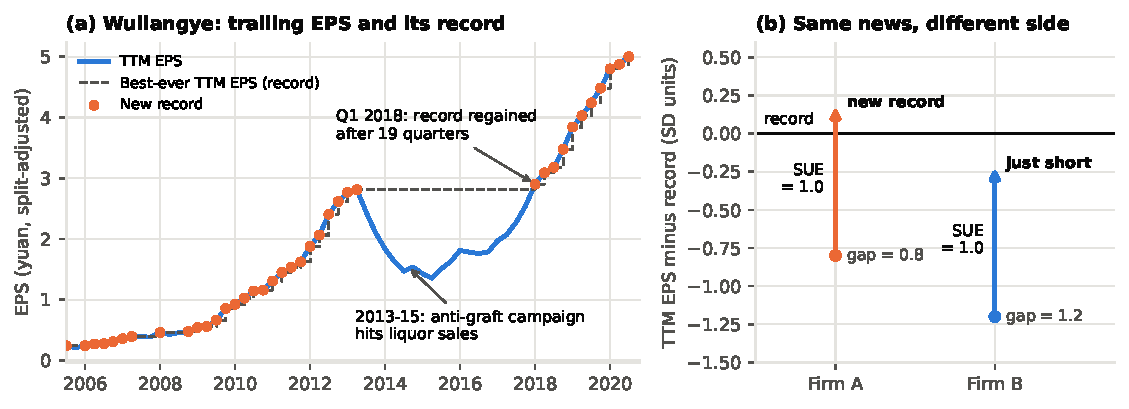
\includegraphics[width=\textwidth]{fig_example.pdf}
\caption{What it takes to set a record. (a) Wuliangye's trailing twelve-month (TTM) EPS, its record (best-ever TTM
EPS, dashed) and the reports that set a new record (dots). The firm regained its 2013 record in its first-quarter
report of 2018, \ExQuarters{} quarters later. (b) Two firms with the same surprise ($\SUE=1$) but different gaps to
their record before the report. Firm A sets a record; firm B falls just short. Our main design compares such firms.}
\label{fig:example}
\end{figure}

\section{Hypotheses}

If investors use the record as a reference point, crossing it should change how they react to the same news. The
literature suggests four testable versions.

\begin{itemize}
\item \textbf{H1 (record premium).} A record is a salient piece of good news and a goal reached
\citep{heath1999,bordalo2012}. Prices jump when earnings just pass the record. If the premium is an overreaction, it
reverses later.
\item \textbf{H2 (anchoring).} Investors anchored on the record are reluctant to believe that earnings will stay above
it, so they underreact to news that pushes earnings past it. Prices then catch up later, as in the 52-week-high
effect \citep{george2004,jang2021}. Returns after the report jump at the record, or rise faster with the margin by
which the record is beaten.
\item \textbf{H3 (attention).} Records attract attention, especially from retail investors \citep{barber2008,seasholes2007}, and
trading volume rises around salient price levels \citep{huddart2009}. Turnover jumps at the record.
\item \textbf{H4 (targeting).} If records matter to investors, managers have an incentive to report just above them,
as they do for zero earnings and last year's earnings \citep{burgstahler1997,degeorge1999,myers2007}. Reports bunch
just above the record.
\end{itemize}

\noindent We also test whether analysts revise their forecasts differently after a record, and whether records predict
future earnings. Under the null hypothesis, the record is irrelevant once we know the news.

\section{Data}

\paragraph{Sample.} We use monthly data on all stocks traded on the Shanghai and Shenzhen exchanges from Thomson
Reuters Datastream and Worldscope, including inactive stocks to avoid survival bias \citep{shumway1997}. The data give
prices, total return indices, trading volume, shares outstanding, book values, the I/B/E/S consensus forecast, and
standalone quarterly EPS with each report's publication date. Our sample contains reports published from 2005 to 2020.
Table~\ref{tab:sample} shows how the \NReports{} reports of \NFirms{} firms are selected.

\paragraph{Records.} Trailing twelve-month EPS ($\TTM$) is the sum of the last four standalone quarters, adjusted for
stock splits and bonus shares so that it is comparable within a firm over time. The \emph{record} is the highest TTM EPS
of all earlier reports; we require at least eight earlier values, so that a record means something, and a positive
record. We measure the news in each report against a seasonal random walk (SRW): expected EPS equals EPS of the same
quarter a year earlier \citep{foster1977,bernard1990}. The scale $\sigma$ is the standard deviation of the firm's last
eight SRW errors, and all distances are in units of $\sigma$:
\begin{equation*}
\SUE = \frac{\mathit{EPS}_q-\mathit{EPS}_{q-4}}{\sigma},\qquad
r = \frac{\TTM_{\mathrm{new}}-\mathrm{record}}{\sigma},\qquad
\gap = \frac{\mathrm{record}-\TTM_{\mathrm{before}}}{\sigma}\geq 0 .
\end{equation*}
Because $\TTM_{\mathrm{new}}-\TTM_{\mathrm{before}}=\mathit{EPS}_q-\mathit{EPS}_{q-4}$, identity \eqref{eq:identity}
holds exactly. A report sets a new record when $r>0$, that is, when the surprise exceeds the gap. We drop
\(451\) exact ties with the record. In the Wuliangye example, $\sigma=\ExSD$ yuan, TTM EPS rose from \ExTTMprev{} to
\ExTTM{} yuan and the old record was \ExRecord{} yuan.

\paragraph{Outcomes.} Returns are monthly and size-adjusted: the stock's return minus the average return of its size
decile. Month 0 is the calendar month of the report, so it contains the reaction to it; we also use the drift over
months $+1$ to $+3$ and $+1$ to $+6$. Abnormal turnover is log monthly turnover minus the firm's average over the
previous year. The analyst revision is the change in the I/B/E/S 12-month-forward consensus EPS from the start of the
report month to the start of the next month, in basis points of the price. We drop April reports here, because the
consensus switches to a new fiscal year in May. Future earnings are the next quarter's SUE and the change in TTM EPS
over the next four quarters, in units of $\sigma$.

\paragraph{Descriptive statistics.} Records are common. \ShareRecords\% of reports set one, and \ShareRecFirms\% of
firms set at least one. Most records extend a run: the previous report was already a record (\emph{extended}
records, Figure~\ref{fig:records}a). Only \ShareRegained\% of reports \emph{regain} a record after falling below it, typically
\QsinceReg{} quarters after it was set. Figure~\ref{fig:records}b shows the distribution of the gap: \ShareAtRec\% of reports
start at their record, and the rest are spread out with a median gap of \MedianGap. Panel (c) shows who sets a record
in the (surprise, gap) plane. Firms at the bottom line ($\gap=0$) set a record whenever $\SUE>0$; firms above it need a
surprise larger than their gap. Table~\ref{tab:desc} shows that record setters are larger and more often covered by
analysts, have much stronger momentum (40\% against 8\% for firms far below their record) and earn higher returns.
Simple comparisons therefore mix the record with good news and good firms.

\begin{table}[t]
\begin{minipage}[t]{0.40\textwidth}
\captionof{table}{Sample construction}\label{tab:sample}
\centering\footnotesize
\resizebox{\linewidth}{!}{\input{\tabpath/tab_sample_flow.tex}}
\note{Reports of A-share firms with a seasonal-random-walk (SRW) surprise. TTM: trailing twelve-month EPS.}
\end{minipage}\hfill
\begin{minipage}[t]{0.57\textwidth}
\captionof{table}{Descriptive statistics by record status}\label{tab:desc}
\centering\footnotesize
\resizebox{\linewidth}{!}{\input{\tabpath/tab_descriptives.tex}}
\note{Means (medians where stated). Extended: new record by a firm at its record. Regained: new record by a firm below
it. Near miss: $-1\leq r<0$. Far below: $r<-1$. Returns are size-adjusted.}
\end{minipage}
\end{table}

\begin{figure}[t]
\centering
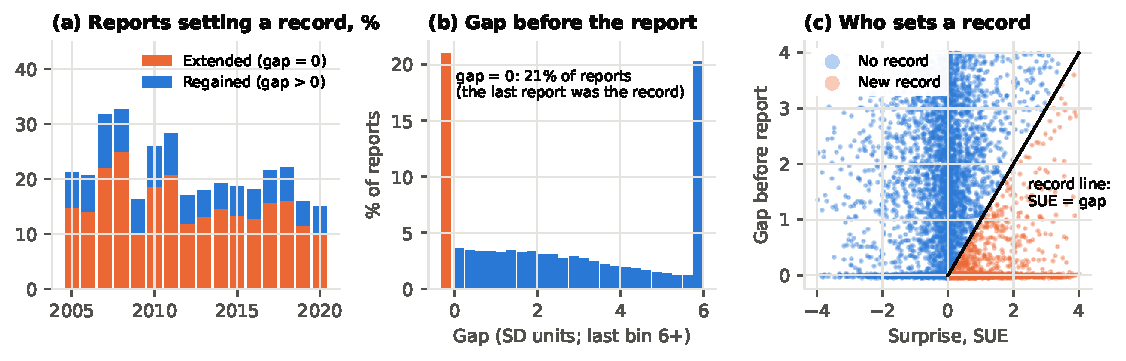
\includegraphics[width=\textwidth]{fig_records.pdf}
\caption{Records in the data. (a) Share of reports that set a new record, by year. (b) Gap to the record before the
report, in units of $\sigma$; the separate bar is the share of reports that start at their record. (c) A random sample
of 5,000 reports by surprise and gap. Records lie below the line $\SUE=\gap$; points at $\gap=0$ are jittered.}
\label{fig:records}
\end{figure}

\section{Methodology}

\paragraph{The naive RD.} The obvious design is a local-linear RD in the distance to the record:
\begin{equation}
y_i = \alpha + \tau D_i + \beta r_i + \kappa D_i r_i + \gamma_{+}\SUE_i^{+} + \gamma_{-}\SUE_i^{-} + \varepsilon_i,
\qquad |r_i|\leq h,
\label{eq:naive}
\end{equation}
where $D_i=1[r_i>0]$ marks a record, the weights fall linearly to zero at the bandwidth $h$ (a triangular kernel), and
$\SUE^{+}$, $\SUE^{-}$ control for good and bad news with separate slopes. The jump $\tau$ tests H1. The kink $\kappa$,
the change in slope at the record, tests the margin version of H2: does the return rise faster with $r$ once earnings
pass the record?

Equation~\eqref{eq:naive} has two problems. For firms at their record, $r=\SUE$, so $D_i r_i=\SUE_i^{+}$. Their
``record kink'' is any change in the slope of the response to news at $\SUE=0$, and returns are known to respond to
news in a nonlinear way \citep{freeman1992}. And kinks are fragile: any curvature in how an outcome varies with $r$
shows up as a kink, because the two linear fits differ in slope even without a break \citep{card2015}. A balance test
on variables fixed before the report reveals both problems.

\paragraph{Main design: the moving cutoff.} We restrict the sample to firms below their record ($\gap>0$) and estimate
\begin{equation}
y_i = \alpha_{b(i)} + \tau D_i + \beta r_i + \kappa D_i r_i + \varepsilon_i,\qquad |r_i|\leq h,
\label{eq:main}
\end{equation}
where $b(i)$ is the surprise bin of report $i$ (bins of 0.25$\sigma$), so each bin has its own intercept. Within a bin
the surprise is almost constant, and by identity~\eqref{eq:identity} the distance to the record varies only through
the gap. The jump $\tau$ therefore compares firms with the same news that end up on different sides of their record
because they started at different distances. The identifying assumption is that, given the surprise, outcomes would
change smoothly with the gap at the point where the gap equals the surprise. This is plausible because the gap is fixed
before the report and the cutoff it implies differs from firm to firm. It would fail if firms could manage earnings to
just pass the record, which the bunching test checks. In the language of the multi-score RD literature, records are
a two-score design in the surprise and the gap with the boundary $\SUE=\gap$, and we estimate the effect along this
boundary \citep{papay2011,reardon2012,wong2013}.

The jump is our main estimate. We use $h=1$ and report $h=2$ and a local-quadratic fit at $h=2$, which corresponds to
the robust bias correction of \citet{calonico2014}; we avoid higher-order polynomials \citep{gelman2019}. We do not
interpret kinks, for the reason given above. Standard errors are clustered by report month and by firm
\citep{petersen2009,cameron2011}.

\paragraph{Firms at their record: a difference in discontinuities.} For firms at their record, the record cannot be
separated from beating last year's quarter within the firm group. We therefore compare them with firms far below their
record ($\gap>h$), for which no surprise within the window sets a record, at the same cutoff $\SUE=0$
\citep{grembi2016}:
\begin{equation}
y_i = \alpha_m + \sum_{g\in\{0,1\}} 1[G_i=g]\,\big(a_g + \tau_g D_i + \beta_g \SUE_i + \kappa_g D_i \SUE_i\big) + \varepsilon_i,
\qquad |\SUE_i|\leq h,
\label{eq:did}
\end{equation}
where now $D_i=1[\SUE_i>0]$, $G_i=1$ for firms at their record, and $\alpha_m$ are report-month fixed effects. The
differences $\tau_1-\tau_0$ and $\kappa_1-\kappa_0$ measure how the response to beating last year's quarter changes
when it also sets a record. The comparison is between two kinds of firms, so we read it together with the evidence on
their fundamentals.

\paragraph{Bunching.} To test H4 we count reports in bins of 0.05$\sigma$ and fit a Poisson regression of the counts
on a polynomial in the running variable on each side of the threshold. The excess mass just above the threshold is
$e^{\hat\delta}-1$, where $\hat\delta$ is the jump in the log density \citep{mccrary2008,cattaneo2020,kleven2016}.

\section{Results}

\subsection{The naive RD finds a kink, but also in firm size}

Table~\ref{tab:naive} reproduces the naive design. Returns do not jump at the record in the report month
(\NaiveJumpA\%, $t=\NaiveJumpAT$) or later. The drift over months $+1$ to $+3$, however, rises faster with $r$ above
the record than below it, by \NaiveKinkD\% per unit of $\sigma$ ($t=\NaiveKinkDT$) at $h=1$ and by \NaiveKinkDtwo\%
($t=\NaiveKinkDtwoT$) at $h=2$. Figure~\ref{fig:naive}a shows the pattern: below the record the drift net of the
surprise is flat or falling; above it, it rises. Read naively, investors underreact to news that pushes earnings past
the record.

Two facts show that this reading is wrong. First, the kink disappears among firms below their record, where the record
and beating last year differ (\NaiveKinkBelow, $t=\NaiveKinkBelowT$; Figure~\ref{fig:naive}b). Second, the same design
applied to variables that are fixed before the report (Panel B) finds a jump and a kink in firm size ($t=\NaiveKinkSizeT$ for
the kink; Figure~\ref{fig:naive}c) and in the previous quarter's surprise ($t=\NaiveKinkPrevT$). The record cannot change
how large a firm was before the report. The design compares firms that differ in more than the record.

\begin{table}[t]
\captionof{table}{The naive regression discontinuity at the record}\label{tab:naive}
\centering\footnotesize
\input{\tabpath/tab_naive.tex}
\vspace{4pt}
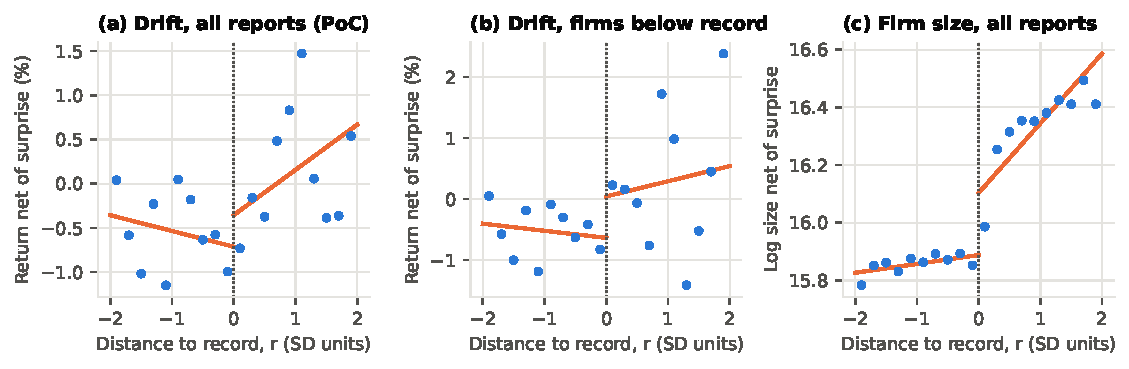
\includegraphics[width=\textwidth]{fig_naive.pdf}
\captionof{figure}{The naive design. Bin means of the outcome net of good and bad surprises, by distance to the
record, with linear fits on each side. (a) Drift, all reports. (b) Drift, firms below their record before the report.
(c) Log market value at the start of the report month, a placebo outcome.}\label{fig:naive}
\note{Equation~\eqref{eq:naive}: local-linear RD with triangular kernel and bandwidth $h$ (in units of $\sigma$),
controlling for $\SUE^{+}$ and $\SUE^{-}$. Panel B uses the same specification with variables fixed before the report
as outcomes. $t$-statistics in parentheses, clustered by report month and firm. *, **, ***: 10\%, 5\%, 1\%.}
\end{table}

\subsection{Main result: the same news, a different side of the record}

Table~\ref{tab:main} reports the moving-cutoff design~\eqref{eq:main} for the \MainNbelow{} reports of firms below
their record. None of the seven outcomes jumps at the record. The announcement-month return is \MainJumpA\% higher
($t=\MainJumpAT$), the drift over months $+1$ to $+3$ is \MainJumpD\% higher ($t=\MainJumpDT$), and the drift over six
months is, if anything, lower (\MainJumpS\%, $t=\MainJumpST$). Trading volume does not rise (\MainJumpTO\%,
$t=\MainJumpTOT$), so a record does not attract attention (H3). Analysts do not revise their forecasts differently
(\MainJumpRev{} bp, $t=\MainJumpRevT$). Nor does a record predict future earnings: the next quarter's surprise and the
next year's earnings growth are, if anything, slightly lower above the record. A record therefore carries no
information about the future beyond the surprise, and the market correctly ignores it. Figure~\ref{fig:main} shows the
raw data: the bin means run smoothly through the record.\footnote{Within a surprise bin, a larger $r$ means a smaller
gap, so the slopes in Figure~\ref{fig:main} show how outcomes vary with the gap. These slopes differ across the record
also for variables fixed before the report, such as firm size, so we do not interpret kinks in this design either.}

How large an effect can we rule out? At $h=2$ the 95\% confidence interval for the announcement-month premium is
[\CIAtwolo, \CIAtwohi]\%. Across all reports, a one-standard-deviation surprise moves the announcement-month return by
\ERCA\%, so a record premium larger than the reaction to a \UBinSDA-standard-deviation surprise is ruled out. For the
three-month drift the interval is [\CIDtwolo, \CIDtwohi]\%.

Table~\ref{tab:balance} supports the design. Characteristics fixed before the report do not jump at the record at
$h=1$; the largest $t$-statistic is \BalMaxT. At $h=2$ the previous quarter's surprise is slightly lower just above the
record ($t=\BalPrevTwoT$), but this disappears with a local-quadratic fit, which suggests curvature rather than a
break; controlling for it leaves the results unchanged (Appendix Table~\ref{tab:rob}). Figure~\ref{fig:bw} shows that
the estimates do not depend on the bandwidth.

\begin{table}[t]
\captionof{table}{Main result: firms below their record, same surprise, different side of the record}\label{tab:main}
\centering\footnotesize
\resizebox{\linewidth}{!}{\input{\tabpath/tab_main.tex}}
\vspace{4pt}
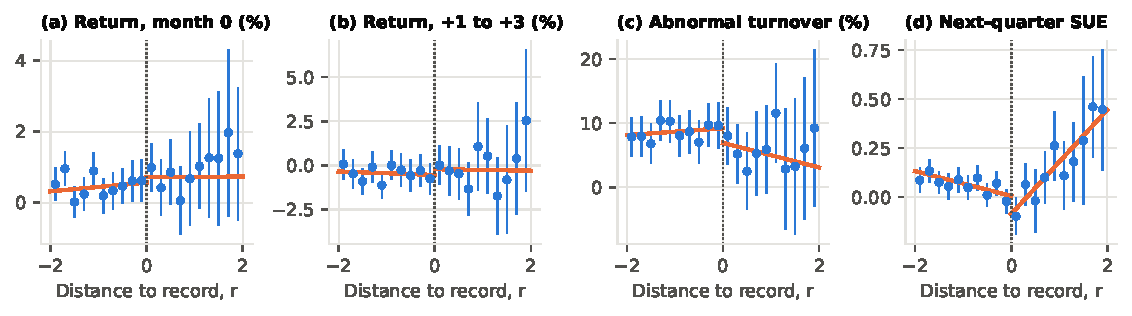
\includegraphics[width=\textwidth]{fig_main.pdf}
\captionof{figure}{Outcomes around the record, firms below their record. Bin means net of surprise-bin effects with
95\% confidence intervals, and local-linear fits on each side.}\label{fig:main}
\note{Equation~\eqref{eq:main}: sample of reports with $\gap>0$; every surprise bin of 0.25$\sigma$ has its own
intercept. Local-linear (or quadratic) RD with triangular kernel and bandwidth $h$. Returns and turnover in \%, analyst
revisions in basis points of the price, EPS growth in units of $\sigma$. $t$-statistics in parentheses, clustered by
report month and firm.}
\end{table}

\begin{table}[t]
\begin{minipage}[t]{0.47\textwidth}
\captionof{table}{Balance: variables fixed before the report}\label{tab:balance}
\centering\footnotesize
\resizebox{\linewidth}{!}{\input{\tabpath/tab_balance.tex}}
\note{Each row re-estimates Equation~\eqref{eq:main} with a characteristic measured before the report as the
outcome.}
\end{minipage}\hfill
\begin{minipage}[t]{0.50\textwidth}
\captionof{figure}{Bandwidth choice}\label{fig:bw}
\centering
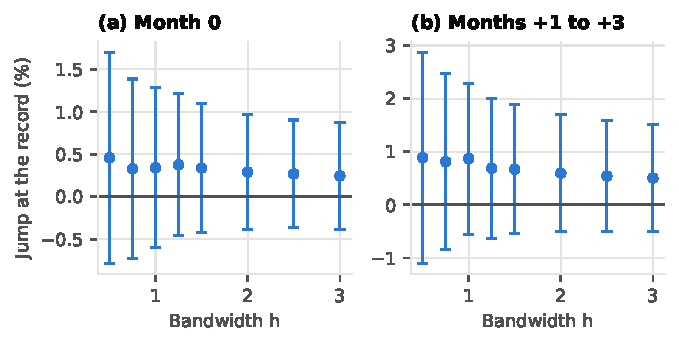
\includegraphics[width=\linewidth]{fig_bandwidth.pdf}
\note{Jump at the record (Equation~\eqref{eq:main}) and 95\% confidence intervals for bandwidths from 0.5 to 3.}
\end{minipage}
\end{table}

\subsection{Firms at their record: different news, the same price response}

Firms whose previous report was a record set a new one whenever they beat last year's quarter. Table~\ref{tab:atrec}
compares their response at $\SUE=0$ with that of firms far below their record (Equation~\eqref{eq:did}), and
Figure~\ref{fig:atrec} plots both. Three results stand out.

First, beating last year's quarter earns no extra premium when it also sets a record. The extra jump is \AtJumpA\%
($t=\AtJumpAT$) in the report month and \AtJumpD\% ($t=\AtJumpDT$) later. This is the same conclusion as in the main
design, from a different comparison.

Second, the news itself differs. For firms far below their record, a one-$\sigma$ surprise predicts a next-quarter
surprise of \SlNfarbad{} when the news is bad and \SlNfargood{} when it is good. For firms at their record, bad news does
not persist at all (\SlNatbad, $t=\SlNatbadT$), while good news persists strongly (\SlNatgood, $t=\SlNatgoodT$;
Figure~\ref{fig:atrec}c). A weak quarter at the peak is usually a blip; a strong quarter at the peak is usually the
start of more.

Third, prices learn this slowly. In the report month, the response of firms at their record has the same shape as that of other firms
(Figure~\ref{fig:atrec}a; the extra kink is \AtKinkA, $t=\AtKinkAT$). Over the next three months, the drift of firms
at their record follows the persistence of their news. Bad news tends to be reversed (\SlDatbad\% per $\sigma$,
$t=\SlDatbadT$), while good news keeps drifting (\SlDatgood\% per $\sigma$, $t=\SlDatgoodT$). The resulting extra kink,
\AtKinkD\% ($t=\AtKinkDT$), is the naive kink of Table~\ref{tab:naive}. It survives when the comparison firms also had
good news in the previous quarter (column 4). Controlling for the realised next-quarter surprise explains about
\AtKinkShare\% of it (column 6), a lower bound because only part of the next reports fall inside the three-month
window.

This is not the anchoring of H2, under which investors would treat the record as special and underreact to news that
passes it. The evidence points the other way: at the announcement, investors treat news at the record like any other
news, even though it is more (or less) persistent, as in the classic drift of \citet{bernard1989,bernard1990}. The
contrast matters for proximity-based evidence such as \citet{jang2021}. Drift that is stronger near the record can
arise because news near the record is more persistent, not because the record is an anchor.

\begin{table}[t]
\captionof{table}{Firms at their record versus firms far below it, at $\SUE=0$}\label{tab:atrec}
\centering\footnotesize
\input{\tabpath/tab_at_record.tex}
\vspace{4pt}
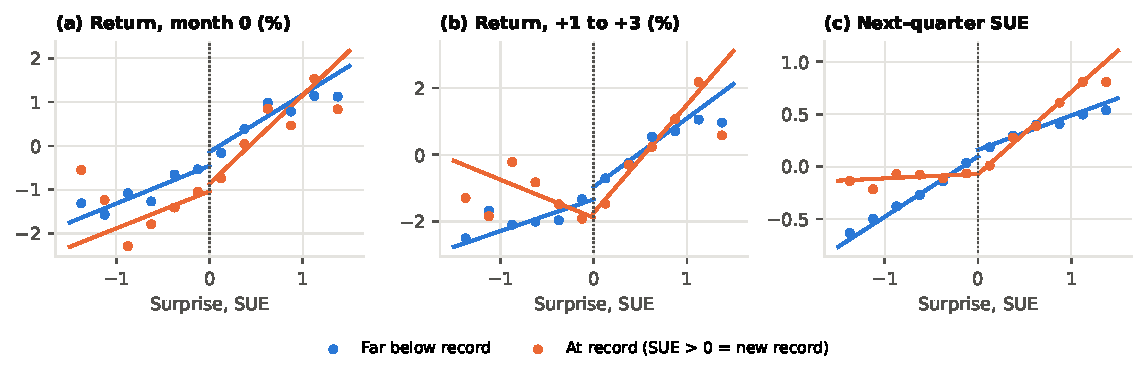
\includegraphics[width=\textwidth]{fig_at_record.pdf}
\captionof{figure}{Response to the surprise by record status. Bin means net of report-month effects and local-linear
fits on each side of $\SUE=0$. For firms at their record, $\SUE>0$ sets a new record.}\label{fig:atrec}
\note{Equation~\eqref{eq:did}: at-record firms ($\gap=0$) versus firms far below their record ($\gap>h$); report-month
fixed effects; triangular kernel. Rows ``Extra'' are the differences between the two groups. Returns in \% per unit of
$\sigma$ (slopes and kinks) or \% (jumps); column 5 in units of the next-quarter SUE. $t$-statistics clustered by report
month and firm.}
\end{table}

\subsection{Do firms manage earnings to set records?}

If records mattered to investors, managers would want to report just above them (H4). Table~\ref{tab:bunch} and
Figure~\ref{fig:bunch} show that they do not. The density of reports is smooth at the record (\BunchRec\%,
$t=\BunchRecT$), also among firms far below their record, where the threshold lies away from the cluster of small
surprises around zero (\BunchFar\%, $t=\BunchFarT$). The test is not powerless. It finds \BunchZero\% excess mass just
above zero TTM earnings ($t=\BunchZeroT$) and \BunchZeroFY\% just above zero annual earnings ($t=\BunchZeroFYT$). In China,
two consecutive annual losses lead to special treatment and, eventually, delisting, and firms manage earnings to avoid
them \citep{chen2004,haw2005}. Firms also bunch just above $\SUE=0$, avoiding a decline from last year's quarter
\citep{burgstahler1997}. They do so whether or not a record is at stake: firms at their record show \BunchSueAt\% excess
mass, and firms below their record that also had good news in the previous quarter show \BunchSueBelow\%.

The density test is less precise near the record than near zero earnings, because the density of $r$ peaks close to
the record. At placebo cutoffs between $-2$ and $2$ the test finds ``effects'' with $|t|$ up to \BunchPlacMaxT. The
estimate at the true record is well inside this range, and in all specifications it is small compared with the
bunching at zero earnings.

\begin{table}[t]
\captionof{table}{Bunching tests}\label{tab:bunch}
\centering\footnotesize
\resizebox{\linewidth}{!}{\input{\tabpath/tab_bunching.tex}}
\vspace{4pt}
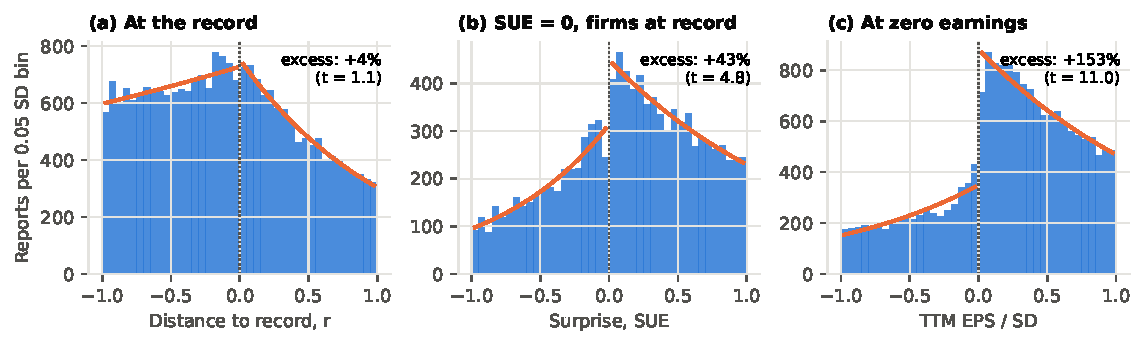
\includegraphics[width=\textwidth]{fig_bunching.pdf}
\captionof{figure}{Reports per bin around three thresholds, with fitted densities on each side. (a) The record, all
reports. (b) Beating last year's quarter, firms at their record. (c) Zero TTM earnings.}\label{fig:bunch}
\note{Poisson regressions of counts in bins of 0.05$\sigma$ (0.025$\sigma$ in row 2) on a polynomial on each side of the
threshold, within the stated window. Excess mass $=e^{\hat\delta}-1$ in \%, with $t$-statistics (robust) in parentheses.}
\end{table}

\subsection{Robustness and heterogeneity}

Figure~\ref{fig:forest} and Appendix Table~\ref{tab:rob} repeat the main design in \RobNrows{} variations. These
include different bandwidths, kernels and surprise bins, surprise-bin-by-year effects, surprises measured with an
out-of-sample XGBoost forecast \citep{chen2016} instead of the SRW, a donut that drops reports within 0.05$\sigma$ of the record, and
controls. Attention constraints should matter most for small firms and firms without analyst coverage, and a record
should be most salient when it is regained after a long time. None of these subsamples shows a robust effect. The
results also hold for three other definitions of a record: the best single quarter, the best year-to-date result for
the same period of earlier years (Chinese firms report cumulative figures) and the best annual result. Across
\RobNtests{} estimates, \RobNsig{} are significant at the 5\% level, about the \RobNsigExp{} that chance alone would
produce. The point estimates for the three-month drift are mostly positive, up to 2.4\%, but significant in only two
of the \RobNrows{} rows. Placebo cutoffs on either side of the record give estimates of the same size as at the
true record.

As a benchmark we apply the same design to the zero-earnings threshold, where Table~\ref{tab:bunch} shows that firms
care a great deal. Here too the announcement return (\ZeroA\%, $t=\ZeroAT$) and turnover (\ZeroTO\%, $t=\ZeroTOT$) jump
only marginally. Monthly data can detect only large threshold effects, a point we return to below.

\begin{figure}[t]
\centering
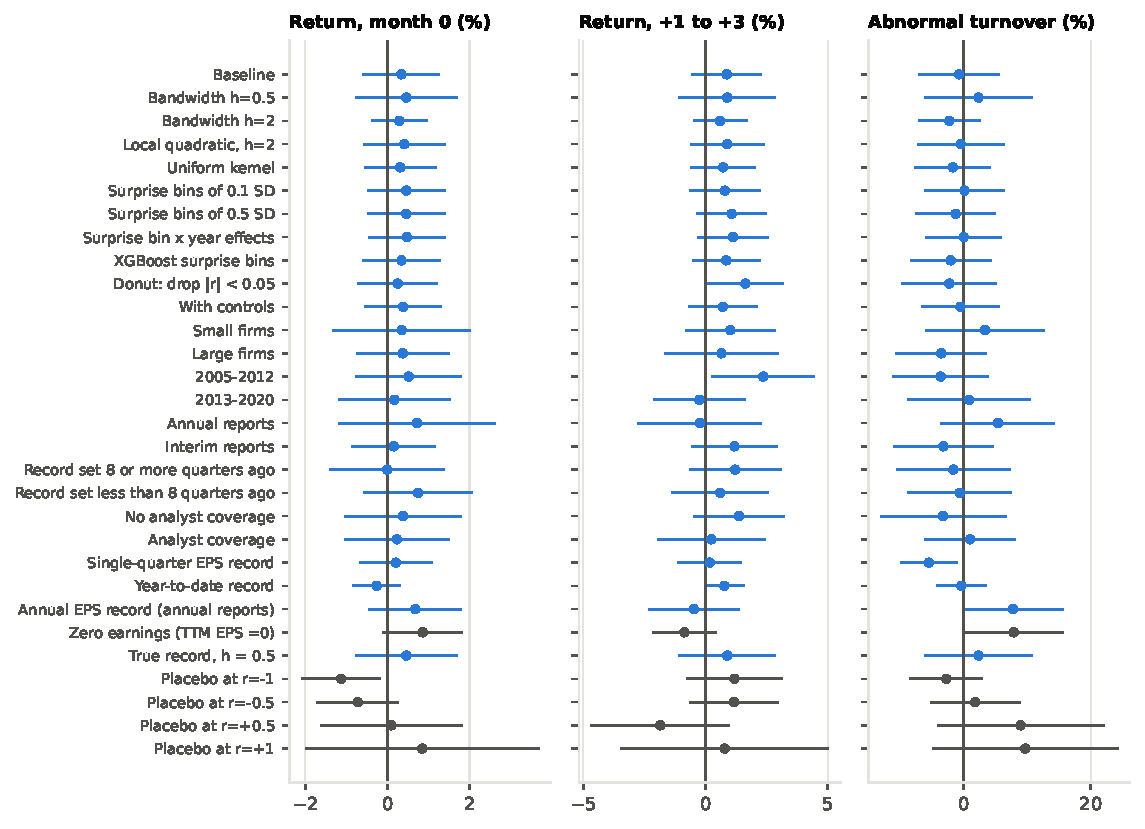
\includegraphics[width=0.93\textwidth]{fig_forest.pdf}
\caption{Robustness. Jump at the record from Equation~\eqref{eq:main} with 95\% confidence intervals, for the
specifications and samples of Appendix Table~\ref{tab:rob}. Grey: benchmark threshold and placebo cutoffs.}
\label{fig:forest}
\end{figure}

\section{Discussion}

Why does the record not matter, when price anchors such as the 52-week high do? Three differences seem important.
First, a price anchor is visible every day on every trading screen, while an earnings record must be computed from
past reports and is reported only when it is broken. Investors see a record headline only after the fact, together with
the news that produced it, and the news is what the price responds to. Second, Chinese reports give cumulative
year-to-date figures and growth on the same period of last year. Trailing records may simply not be the numbers
investors look at. Our results for year-to-date and annual records suggest that this is not the whole story. Third, the
record carries no information about future earnings beyond the surprise (Table~\ref{tab:main}), so there is nothing for
an informed investor to trade on, and nothing for managers to gain from reaching it.

Our evidence has limits. Monthly returns cannot detect a premium that appears and disappears within a few days, and
the benchmark at zero earnings shows that our design detects only large threshold effects in prices and volume. The
bound we report is therefore a bound on effects that last at least until the end of the report month. Records are
defined on split-adjusted EPS. Headlines usually refer to net profit, which differs from EPS when firms issue shares,
so some firms are misclassified close to the record; such errors would weaken a true jump. Finally, the comparison of
firms at their record with firms far below it is between two kinds of firms. We use it to describe how their news
differs, not to identify a causal effect of the record.

\section{Conclusion}

Record earnings look like an ideal reference point, and a simple RD seems to confirm that investors anchor on them.
The confirmation is an artefact. Because trailing earnings move by exactly the surprise, the distance to the record is
the surprise minus the pre-report gap, and most records are set by firms that were already at their record. Using the
gap, which is fixed before the report, to compare firms with the same news on either side of their record, we find
that a new record moves neither prices, nor trading, nor analysts, nor future earnings, and that managers do not
manage earnings to reach it. What does differ at the record is the persistence of news, which prices learn slowly.
The method carries over to any threshold defined by a running maximum: before reading a break at the maximum as
behaviour, ask whether the maximum was crossed by the news itself.

\setstretch{1.0}
\small
\begin{thebibliography}{99}
\bibitem[Allen et~al.(2017)]{allen2017} Allen, E.~J., Dechow, P.~M., Pope, D.~G., Wu, G., 2017. Reference-dependent
preferences: Evidence from marathon runners. \emph{Management Science} 63(6), 1657--1672.
\bibitem[Baker et~al.(2012)]{baker2012} Baker, M., Pan, X., Wurgler, J., 2012. The effect of reference point prices on
mergers and acquisitions. \emph{Journal of Financial Economics} 106(1), 49--71.
\bibitem[Barber and Odean(2008)]{barber2008} Barber, B.~M., Odean, T., 2008. All that glitters: The effect of attention
and news on the buying behavior of individual and institutional investors. \emph{Review of Financial Studies} 21(2),
785--818.
\bibitem[Barth et~al.(1999)]{barth1999} Barth, M.~E., Elliott, J.~A., Finn, M.~W., 1999. Market rewards associated with
patterns of increasing earnings. \emph{Journal of Accounting Research} 37(2), 387--413.
\bibitem[Bernard and Thomas(1989)]{bernard1989} Bernard, V.~L., Thomas, J.~K., 1989. Post-earnings-announcement drift:
Delayed price response or risk premium? \emph{Journal of Accounting Research} 27(Supplement), 1--36.
\bibitem[Bernard and Thomas(1990)]{bernard1990} Bernard, V.~L., Thomas, J.~K., 1990. Evidence that stock prices do not
fully reflect the implications of current earnings for future earnings. \emph{Journal of Accounting and Economics}
13(4), 305--340.
\bibitem[Bordalo et~al.(2012)]{bordalo2012} Bordalo, P., Gennaioli, N., Shleifer, A., 2012. Salience theory of choice
under risk. \emph{Quarterly Journal of Economics} 127(3), 1243--1285.
\bibitem[Burgstahler and Dichev(1997)]{burgstahler1997} Burgstahler, D., Dichev, I., 1997. Earnings management to avoid
earnings decreases and losses. \emph{Journal of Accounting and Economics} 24(1), 99--126.
\bibitem[Calonico et~al.(2014)]{calonico2014} Calonico, S., Cattaneo, M.~D., Titiunik, R., 2014. Robust nonparametric
confidence intervals for regression-discontinuity designs. \emph{Econometrica} 82(6), 2295--2326.
\bibitem[Cameron et~al.(2011)]{cameron2011} Cameron, A.~C., Gelbach, J.~B., Miller, D.~L., 2011. Robust inference with
multiway clustering. \emph{Journal of Business \& Economic Statistics} 29(2), 238--249.
\bibitem[Card et~al.(2015)]{card2015} Card, D., Lee, D.~S., Pei, Z., Weber, A., 2015. Inference on causal effects in a
generalized regression kink design. \emph{Econometrica} 83(6), 2453--2483.
\bibitem[Carpenter et~al.(2021)]{carpenter2021} Carpenter, J.~N., Lu, F., Whitelaw, R.~F., 2021. The real value of
China's stock market. \emph{Journal of Financial Economics} 139(3), 679--696.
\bibitem[Cattaneo et~al.(2020)]{cattaneo2020} Cattaneo, M.~D., Jansson, M., Ma, X., 2020. Simple local polynomial
density estimators. \emph{Journal of the American Statistical Association} 115(531), 1449--1455.
\bibitem[Chen and Guestrin(2016)]{chen2016} Chen, T., Guestrin, C., 2016. XGBoost: A scalable tree boosting system.
\emph{Proceedings of the 22nd ACM SIGKDD Conference}, 785--794.
\bibitem[Chen and Yuan(2004)]{chen2004} Chen, K.~C.~W., Yuan, H., 2004. Earnings management and capital resource
allocation: Evidence from China's accounting-based regulation of rights issues. \emph{The Accounting Review} 79(3),
645--665.
\bibitem[Degeorge et~al.(1999)]{degeorge1999} Degeorge, F., Patel, J., Zeckhauser, R., 1999. Earnings management to
exceed thresholds. \emph{Journal of Business} 72(1), 1--33.
\bibitem[Foster(1977)]{foster1977} Foster, G., 1977. Quarterly accounting data: Time-series properties and
predictive-ability results. \emph{The Accounting Review} 52(1), 1--21.
\bibitem[Freeman and Tse(1992)]{freeman1992} Freeman, R.~N., Tse, S.~Y., 1992. A nonlinear model of security price
responses to unexpected earnings. \emph{Journal of Accounting Research} 30(2), 185--209.
\bibitem[Gelman and Imbens(2019)]{gelman2019} Gelman, A., Imbens, G., 2019. Why high-order polynomials should not be
used in regression discontinuity designs. \emph{Journal of Business \& Economic Statistics} 37(3), 447--456.
\bibitem[George and Hwang(2004)]{george2004} George, T.~J., Hwang, C.-Y., 2004. The 52-week high and momentum investing.
\emph{Journal of Finance} 59(5), 2145--2176.
\bibitem[Graham et~al.(2005)]{graham2005} Graham, J.~R., Harvey, C.~R., Rajgopal, S., 2005. The economic implications of
corporate financial reporting. \emph{Journal of Accounting and Economics} 40(1--3), 3--73.
\bibitem[Grembi et~al.(2016)]{grembi2016} Grembi, V., Nannicini, T., Troiano, U., 2016. Do fiscal rules matter?
\emph{American Economic Journal: Applied Economics} 8(3), 1--30.
\bibitem[Haw et~al.(2005)]{haw2005} Haw, I.-M., Qi, D., Wu, D., Wu, W., 2005. Market consequences of earnings management
in response to security regulations in China. \emph{Contemporary Accounting Research} 22(1), 95--140.
\bibitem[Heath et~al.(1999)]{heath1999} Heath, C., Larrick, R.~P., Wu, G., 1999. Goals as reference points.
\emph{Cognitive Psychology} 38(1), 79--109.
\bibitem[Huddart et~al.(2009)]{huddart2009} Huddart, S., Lang, M., Yetman, M.~H., 2009. Volume and price patterns around
a stock's 52-week highs and lows: Theory and evidence. \emph{Management Science} 55(1), 16--31.
\bibitem[Jang and Lee(2021)]{jang2021} Jang, J., Lee, E., 2021. Do record earnings affect market reactions to earnings
news? \emph{Review of Quantitative Finance and Accounting} 56(4), 1259--1287.
\bibitem[Jones et~al.(2025)]{jones2025} Jones, C.~M., Shi, D., Zhang, X., Zhang, X., 2025. Retail trading and return
predictability in China. \emph{Journal of Financial and Quantitative Analysis} 60(1), 68--104.
\bibitem[Kahneman and Tversky(1979)]{kahneman1979} Kahneman, D., Tversky, A., 1979. Prospect theory: An analysis of
decision under risk. \emph{Econometrica} 47(2), 263--291.
\bibitem[Kleven(2016)]{kleven2016} Kleven, H.~J., 2016. Bunching. \emph{Annual Review of Economics} 8, 435--464.
\bibitem[K\H{o}szegi and Rabin(2006)]{koszegi2006} K\H{o}szegi, B., Rabin, M., 2006. A model of reference-dependent
preferences. \emph{Quarterly Journal of Economics} 121(4), 1133--1165.
\bibitem[Li and Yu(2012)]{li2012} Li, J., Yu, J., 2012. Investor attention, psychological anchors, and stock return
predictability. \emph{Journal of Financial Economics} 104(2), 401--419.
\bibitem[McCrary(2008)]{mccrary2008} McCrary, J., 2008. Manipulation of the running variable in the regression
discontinuity design: A density test. \emph{Journal of Econometrics} 142(2), 698--714.
\bibitem[Myers et~al.(2007)]{myers2007} Myers, J.~N., Myers, L.~A., Skinner, D.~J., 2007. Earnings momentum and earnings
management. \emph{Journal of Accounting, Auditing \& Finance} 22(2), 249--284.
\bibitem[Papay et~al.(2011)]{papay2011} Papay, J.~P., Willett, J.~B., Murnane, R.~J., 2011. Extending the
regression-discontinuity approach to multiple assignment variables. \emph{Journal of Econometrics} 161(2), 203--207.
\bibitem[Petersen(2009)]{petersen2009} Petersen, M.~A., 2009. Estimating standard errors in finance panel data sets:
Comparing approaches. \emph{Review of Financial Studies} 22(1), 435--480.
\bibitem[Pope and Simonsohn(2011)]{pope2011} Pope, D., Simonsohn, U., 2011. Round numbers as goals: Evidence from
baseball, SAT takers, and the lab. \emph{Psychological Science} 22(1), 71--79.
\bibitem[Reardon and Robinson(2012)]{reardon2012} Reardon, S.~F., Robinson, J.~P., 2012. Regression discontinuity designs
with multiple rating-score variables. \emph{Journal of Research on Educational Effectiveness} 5(1), 83--104.
\bibitem[Seasholes and Wu(2007)]{seasholes2007} Seasholes, M.~S., Wu, G., 2007. Predictable behavior, profits, and
attention. \emph{Journal of Empirical Finance} 14(5), 590--610.
\bibitem[Shumway(1997)]{shumway1997} Shumway, T., 1997. The delisting bias in CRSP data. \emph{Journal of Finance} 52(1),
327--340.
\bibitem[Wong et~al.(2013)]{wong2013} Wong, V.~C., Steiner, P.~M., Cook, T.~D., 2013. Analyzing regression-discontinuity
designs with multiple assignment variables: A comparative study of four estimation methods. \emph{Journal of
Educational and Behavioral Statistics} 38(2), 107--141.
\end{thebibliography}

\normalsize
\appendix
\section*{Appendix}
\setcounter{table}{0}
\renewcommand{\thetable}{A\arabic{table}}

\begin{table}[h]
\captionof{table}{Robustness, heterogeneity, other record definitions and placebos}\label{tab:rob}
\centering\footnotesize
\resizebox{\linewidth}{!}{\input{\tabpath/tab_robustness.tex}}
\note{Each row re-estimates the jump at the record of Equation~\eqref{eq:main} (firms below their record, $h=1$,
surprise bins of 0.25$\sigma$, triangular kernel) unless stated otherwise; $t$-statistics in parentheses, clustered by
report month and firm. Small and large firms split at the yearly median of size. Other record definitions use all
reports with that definition and drop firms exactly at their record. The zero-earnings row uses TTM EPS$/\sigma$ as the
running variable. Placebo rows use reports on one side of the record only, with a bandwidth of 0.5.}
\end{table}

\end{document}
